\section{$\SU(N)$ 理论的 Argyres-Seiberg-Gaiotto 对偶}\label{sec:duality}
\subsection{含有 $N_f=2N$ 个味的 $\SU(N)$ 理论的 S 对偶，第一部分}\index{FullPuncture@完全穿孔|hyperpage}\index{SimplePuncture@简单穿孔|hyperpage}\index{SUNConformal@含 $2N$ 个味的 $\SU(N)$ 理论|hyperpage}
\subsubsection{曲线的改写}
上一节已经知道，含有 $2N$ 个味的 $\SU(N)$ 理论的曲线为
\begin{equation}
\frac{\prod_{i=1}^N(\tilde x-\tilde\mu_i)}{\tilde z}
+f\prod_{i=1}^N(\tilde x-\tilde\mu'_i)\tilde z
=\tilde x^N+\tilde u_2\tilde x^{N-2}+\cdots+u_N\label{step1}
\end{equation}
其中 $f$ 是复数；微分为 $\tilde\lambda=\tilde xdz/z$。这一理论是超共形的，$f$ 是紫外耦合常数 $\tau_{UV}$ 的函数。我们希望理解这一理论的强耦合极限。

与第 \ref{sec:gaiotto} 节中的做法一样，用 Seiberg-Witten 微分 $\lambda$ 将曲线改写成如下形式较为方便：
\begin{equation}
\lambda^N+\phi_2(z)\lambda^{N-2}+\cdots+\phi_N(z)=0.\label{suN-gaiotto}
\end{equation}
从式 \eqref{step1} 出发，首先按 $\tilde x$ 的相同幂次合并各项：
\begin{equation}
(1-\frac1{\tilde z}-f\tilde z)\tilde x^N
+\heartsuit_1\tilde x^{N-1}+\heartsuit_2\tilde x^{N-2}+\cdots+\heartsuit_N=0
\end{equation}
其中
\begin{equation}
\heartsuit_1=\frac{\sum\tilde\mu_i}{\tilde z}+f\tilde z\sum\tilde\mu'_i.
\end{equation}
将整个方程除以 $(1-1/\tilde z-f\tilde z)$，并定义 $x=\tilde x+\heartsuit_1/(1-1/\tilde z-f\tilde z)/N$。此时有
\begin{equation}
x^N+\clubsuit_2x^{N-2}+\cdots+\clubsuit_N=0
\end{equation}
其中，由于从 $\tilde x$ 到 $x$ 的平移，$\clubsuit_k$ 在 $1-1/\tilde z-f\tilde z=0$ 的两个零点 $\tilde z_{1,2}$ 处具有 $k$ 阶极点。令 $z=\tilde z/\tilde z_1$，使一个零点现在位于 $1$，另一个位于 $q=\tilde z_2/\tilde z_1$。

引入 $\lambda=xdz/z$，便得到式 \eqref{suN-gaiotto} 形式的方程；$\phi_k(z)$ 在 $z=0$、$q$、$1$ 和 $\infty$ 处具有至多 $k$ 阶的极点。考虑所有 $\tilde\mu_i$ 与 $\tilde\mu'_i$ 都取一般值的情形，并假设 $q\ll1$。此时，很容易确定 $\lambda$ 在各奇点附近的行为。由于求解的是 $N$ 次方程，每个奇点处有 $N$ 个留数，分别为
\begin{equation}
\begin{array}{llllr@{\qquad}l@{}llll}
\mu_1,&\mu_2,&\ldots,&\mu_{N-1},&\mu_N,&z&\sim0,&\\
\mu,&\mu,&\ldots,&\mu,&(1-N)\mu,&z&\sim q,&\\
\mu',&\mu',&\ldots,&\mu',&(1-N)\mu',&z&\sim1,&\\
\mu'_1,&\mu'_2,&\ldots,&\mu'_{N-1},&\mu'_N,&z&\sim\infty.
\end{array}\label{simple-full-massive-condition}
\end{equation}
这里
\begin{align}
\mu_i&=\tilde\mu_i-\frac1N\sum_i\tilde\mu_i+O(q),&\sum\mu_i=0;\\
\mu&=\frac1N\sum_i\tilde\mu_i+O(q)
\end{align}
$\mu'_i$、$\mu'$ 也有类似关系。注意，$\mu_i$ 与 $\mu$ 是进入 BPS 质量公式的质量参数。我们发现，它们通过有限重整化与参数 $\tilde\mu_i$ 相联系。

当 $N=2$ 时，四个穿孔处的留数结构属于同一类型，因为它们都具有 $(m,-m)$ 的形式。对于 $N>2$，$z=0,\infty$ 处的留数结构与 $z=q,1$ 处的结构不同。前者具有 $(m_1,\ldots,m_N)$ 的形式，满足 $\sum m_i=0$；后者则具有 $m(1,1,\ldots,1-N)$ 的形式。

考虑完全无质量的情形也很有启发，即对所有 $i$ 都有 $\tilde\mu_i=\tilde\mu'_i=0$。原来的曲线只是
\begin{equation}
\frac{x^N}z+fx^Nz=x^N+u_2x^{N-2}+\cdots+u_N.
\end{equation}
作与上面相同的处理，得到
\begin{equation}
\phi_k(z)=\frac{u_k}{(z-q)(z-1)}\frac{dz^k}{z^{k-1}}.
\end{equation}
因此，
\begin{equation}
\begin{array}{rll}
\text{$\phi_k(z)$ 的极点阶数为}&k-1&\text{当 $z=0,\infty$ 时},\\
\text{$\phi_k(z)$ 的极点阶数为}&1&\text{当 $z=q,1$ 时}.
\end{array}\label{simple-full-condition}
\end{equation}
再次观察到，当 $N=2$ 时，各处极点的行为都相同；而当 $N>2$ 时，$z=0,\infty$ 处的行为与 $z=1,q$ 处的行为不同。

\begin{figure}[h]
\[
\inc{suN-2N}
\]
\caption{含有 $2N$ 个味的 $\SU(N)$ 理论的紫外曲线。\label{fig:suNgaiotto}}
\end{figure}

系统中有 $2N$ 个质量项。首先将它们分为编码在 $z\sim0$ 区域中的 $N$ 个质量项，以及编码在 $z\sim\infty$ 区域中的另外 $N$ 个质量项。相应地，从味对称性 $\U(2N)$ 出发，将它分解为 $\U(N)\times\U(N)$。再将每个 $\U(N)$ 分解为 $\SU(N)$ 与 $\U(1)$。合在一起，使用的味对称性分解为
\begin{equation}
\U(2N)\supset\U(N)\times\U(N)
\simeq[\SU(N)_A\times\U(1)_B]\times[\U(1)_C\times\SU(N)_D].
\end{equation}
$\lambda$ 在 $z=0$ 处穿孔 $A$ 和 $z=\infty$ 处穿孔 $D$ 的留数，分别编码 $\SU(N)_{A,D}$ 的质量项；而在 $z=q$ 处穿孔 $B$ 和 $z=1$ 处穿孔 $C$ 的留数，编码 $\U(1)_{B,C}$ 的质量项；可与式 \eqref{simple-full-massive-condition} 比较。

于是，我们说 $z=0$ 处的奇点带有 $\SU(N)$ 对称性，$z=q$ 处的奇点带有 $\U(1)$ 对称性，$z=1$、$=\infty$ 处也类似。这一情形可以画成图 \ref{fig:suNgaiotto} 的样子。将 $z=0,\infty$ 处的穿孔称为完全穿孔，将 $z=q,1$ 处的穿孔称为简单穿孔。从六维观点看，它们是沿闵可夫斯基空间 $\bR^{3,1}$ 延展的四维缺陷对象，其上带有各自的味对称性。
% [Tutor Note: 原文两处把第二个奇点的坐标写成 "$=\infty$"（漏写 $z$）：p.143 "those at $z=1$, $=\infty$" 与 p.146 "two at $z=0$, $=\infty$"，均应读作 $z=\infty$。正文照原文排版。]

当 $N=2$ 时，原来的对称性不只是 $\U(2)$，而是 $\SO(4)$。相应地，分解 $\U(2)\simeq\SU(2)\times\U(1)$ 增强为如下结构：
\begin{equation}
\begin{array}{ccccc}
\SO(4)&\supset&\SU(2)&\times&\SU(2)\\
\cup&&\rotatebox{90}{$=$}&&\cup\\
\U(2)&\supset&\SU(2)&\times&\U(1)
\end{array}
\end{equation}
因此，穿孔类型之间的区别消失了。

\subsubsection{弱耦合极限}
\begin{figure}[h]
\[
\inc{suN-2N-weak}
\]
\caption{弱耦合极限。\label{fig:weakSUN}}
\end{figure}
显然，在弱耦合区域有 $f\sim q\sim e^{2\pi i\tau_{UV}}$，见图 \ref{fig:weakSUN}。当耦合极弱时，可以认为左侧的四穿孔球面由两个三穿孔球面组成。在连接两者的管状区域中，$\lambda$ 的行为基本上仅由
\begin{equation}
\phi_k(z)\sim u_k\frac{dz^k}{z^k}.
\end{equation}
给出。写成
\begin{equation}
\prod(x-a_i)=x^N+u_2x^{N-2}+\cdots+u_N,
\end{equation}
可知 $\lambda$ 在管状区域中的留数为 $a_1,\ldots,a_N$。因此，将两个球面分离之后，得到完全穿孔。

所得到的三穿孔球面带有一个简单穿孔和两个完全穿孔。因此，它应具有 $\U(1)\times\SU(N)\times\SU(N)$ 对称性。四穿孔球面代表含有 $2N$ 个味的 $\SU(N)$ 理论。管状区域承载 $\SU(N)$ 矢量多重态。于是，每个三穿孔球面就代表 $N$ 个味，即超多重态 $(Q_i^a,\tilde Q^i_a)$，其中 $a,i=1,\ldots,N$。两个 $\SU(N)$ 对称性可以分别与作用于指标 $a$ 和 $i$ 的对称性对应起来，而 $\U(1)$ 对称性使 $Q$ 的荷为 $+1$，$\tilde Q$ 的荷为 $-1$。

图 \ref{fig:suNgaiotto} 中含有 $2N$ 个味的 $\SU(N)$ 理论的紫外曲线，由这种三穿孔球面的两个副本组成。$2N$ 个超多重态被分成在 $\SU(N)_A$ 和 $\U(1)_B$ 下带荷的 $N$ 个超多重态 $(Q_i^a,\tilde Q^i_a)$，以及在 $\SU(N)_D$ 和 $\U(1)_C$ 下带荷的另外 $N$ 个超多重态 $(Q'{}_i^a,\tilde Q'{}^i_a)$。

\begin{figure}[h]
\[
\inc{suN-2N-S}
\]
\caption{含有 $2N$ 个味的 $\SU(N)$ 理论的 S 对偶。\label{fig:SUN-S}}
\end{figure}

\subsubsection{一个强耦合极限}
考虑 $q\to\infty$ 时会发生什么。如图 \ref{fig:SUN-S} 所示，最终只是交换了穿孔 $B$ 与 $C$，同时通过 $q'=1/q$ 重定义耦合 $q$。这意味着，这一强耦合极限实际上是另一个含有 $2N$ 个味的弱耦合 $\SU(N)$ 规范理论。这一次，$2N$ 个超多重态被分成 $N$ 个超多重态 $(q_i^a,\tilde q^i_a)$ 和另外 $N$ 个超多重态 $(q'{}_i^a,\tilde q'{}^i_a)$，不过要注意，前 $N$ 个在 $\SU(N)_A$ 和 $\U(1)_C$ 下带荷，后 $N$ 个在 $\SU(N)_D$ 和 $\U(1)_B$ 下带荷。正如第 \ref{sec:su2-4-strong} 小节中对含有四个味的 $\SU(2)$ 理论所学到的，从原理论的观点看，新夸克是磁性的。

\begin{figure}[h]
\[
\inc{suN-2N-AS}
\]
\caption{含有 $2N$ 个味的 $\SU(N)$ 理论的另一个极限。\label{fig:Argyres-Seiberg}}
\end{figure}
我们也希望理解极限 $q\to1$。需要按图 \ref{fig:Argyres-Seiberg} 所示的方式拆分四穿孔球面。但穿孔的配置并不是我们已经熟悉的情形：一侧有两个完全穿孔，另一侧有两个简单穿孔。在回答这一极限中会发生什么之前，需要进一步了解六维构造。

\subsection{$\SU(N)$ 箭图理论与驯服穿孔}\label{sec:tame}
\subsubsection{箭图规范理论}\index{QuiverGaugeTheory@箭图规范理论|hyperpage}
为此，引入一种用于 $\cN{=}2$ 规范理论的新图示记号。这一记号与第 \ref{sec:trivalent} 小节引入的三价图记号相关，但并不相同。

一张图由内部写有整数的方框和圆圈，以及连接方框与圆圈的边组成。标有 $N$ 的方框代表 $\U(N)$ 味对称性，标有 $N$ 的圆圈代表 $\SU(N)$ 规范对称性。连接两个分别标有 $N$ 和 $M$ 的对象的边，代表超多重态 $(Q_i^a,\tilde Q^i_a)$，其中 $i=1,\ldots,N$，$j=1,\ldots,M$。它们处于 $\SU(N)$ 与 $\SU(M)$ 基本表示的张量积中，称为双基本表示超多重态。这样一张图就指定了一个 $\cN{=}2$ 规范理论。这类理论通常称为箭图规范理论。

\begin{figure}[h]
\[
\inc{suN-quiver}
\]
\caption{$\SU(N)$ 箭图理论。\label{fig:SUN-quiver}}
\end{figure}

最简单的情形，是所有方框和圆圈中都写着相同的数 $N$，见图 \ref{fig:SUN-quiver}。图中的第一个只是一个双基本表示超多重态。第二个是含有 $2N$ 个味的 $\SU(N)$ 理论。最后一个是 $\SU(N)_1\times\SU(N)_2$ 理论，其中
\begin{itemize}
\item 有一个 $\SU(N)_1\times\SU(N)_2$ 的双基本表示超多重态；
\item 有 $N$ 个 $\SU(N)_1$ 的基本表示超多重态；
\item 有 $N$ 个 $\SU(N)_2$ 的基本表示超多重态。
\end{itemize}
注意，$\SU(N)_1$ 和 $\SU(N)_2$ 的 $\beta$ 函数都为零。

综合迄今掌握的知识，就可以得到它们的 Seiberg-Witten 解。具体而言，每条边对应 $\SU(N)\times\SU(N)$ 的双基本表示超多重态，而我们知道，它来自 $\SU(N)$ 型六维理论的一个三穿孔球面，带有两个完全穿孔和一个简单穿孔。因此，只需为每条边准备一个这样的球面，并用管将完全穿孔两两连接起来。例如，图 \ref{fig:SUN-quiver} 中第三个理论的 Seiberg-Witten 解为
\begin{equation}
\lambda^N+\phi_2(z)\lambda^{N-2}+\cdots+\phi_N(z)=0\label{qwerty}
\end{equation}
其中 $\phi_k(z)$ 有五个奇点：$z=0$、$=\infty$ 处的两个是完全穿孔，$z=1$、$q$ 和 $qq'$ 处的另外三个是简单穿孔。

为简单起见，假设所有质量参数都为零。那么，由式 \eqref{simple-full-condition} 中给出的奇点极点阶数条件，场 $\phi_k(z)$ 被唯一确定为
\begin{equation}
\phi_k(z)=\frac{u_k^{(1)}z+u_k^{(2)}}{(z-1)(z-q)(z-qq')}\frac{dz^k}{z^{k-1}}.
\end{equation}
读者应当检验它在 $z=\infty$ 处具有正确的行为。这一理论是超共形的，因为 $\SU(1)_1$ 和 $\SU(2)_2$ 的单圈 $\beta$ 函数都为零。这也体现为如下事实：可以自然地给 Seiberg-Witten 曲线 \eqref{qwerty} 中出现的变量赋予标度维数。微分 $\lambda$ 应具有标度维数 $1$，因为它的积分给出 BPS 质量公式：$[\lambda]=1$。随后令 $[z]=0$、$[\phi_k]=k$。这意味着，$u_k^{(i=1,2)}$ 应当是两个标度维数为 $k$ 的库仑支算符。确实，我们处理的是一个超共形的 $\SU(N)^2$ 规范理论，而对于 $k=2,\ldots,N$，恰好各有一个标度维数为 $k$ 的库仑支算符。
% [Tutor Note: p.146 原文 "both $\SU(1)_1$ and $\SU(2)_2$ have zero one-loop beta function" 与本小节前文构造的 "$\SU(N)_1\times\SU(N)_2$ 理论"不符：两群应为 $\SU(N)_1$ 与 $\SU(N)_2$。判据：本句断言两群的单圈 $\beta$ 函数为零，这要求每个 $\SU(N)$ 群耦合 $2N$ 个基本表示超多重态（这正是前文构造该理论时的条件）；若按字面取 $\SU(1)$ 与 $\SU(2)$，$\beta$ 函数并不为零。正文照原文排版。]

\subsubsection{$\cN{=}2^*$ 理论}
\begin{figure}[h]
\[
\inc{suN-adj}
\]
\caption{$\SU(N)$ 加伴随表示：$\cN{=}2^*$ 理论。\label{fig:N2*}}
\end{figure}

如果只取一个双基本表示超多重态 $(Q_i^a,\tilde Q^a_i)$，并将一个 $\SU(N)$ 规范多重态耦合到两个指标，就出现一个颇为退化的情形，见图 \ref{fig:N2*}。此时，$N\times N$ 个超多重态分量表现为一个伴随表示加一个单态。单态部分完全退耦，因此这一理论本质上就是含有伴随表示超多重态的 $\SU(N)$ 规范理论。无质量时，它是 $\cN{=}4$ 超杨--米尔斯理论；有质量时，则称为 $\cN{=}2^*$ 理论。取一个三穿孔球面，将两个完全穿孔连接起来，就得到 Seiberg-Witten 解。最终得到一个带有一个简单穿孔的环面。这一解最初在文献 \cite{Donagi:1995cf} 中求得，读者可参阅该文了解细节。

\subsubsection{线性箭图理论}\index{LinearQuiver@线性箭图|hyperpage}\index{QuiverTail@箭图尾部|hyperpage}\index{YoungDiagram@杨图|hyperpage}\index{Partition@分拆|hyperpage}
迄今为止，我们学会了如何求解图 \ref{fig:SUN-quiver} 所示的规范理论。它们的规范群为
\begin{equation}
\SU(N)\times\cdots\times\SU(N)\times\cdots\times\SU(N)
\end{equation}
相邻的 $\SU(N)$ 群之间有双基本表示超多重态，首尾的 $\SU(N)$ 群还各有额外的 $N$ 个味。所有 $\SU(N)$ 群的 $\beta$ 函数都为零。

考虑对这类理论作一个小的推广。规范群具有如下形式：
\begin{equation}
\SU(N)\times\cdots\times\SU(N)\times\SU(N_k)\times\SU(N_{k-1})\times\cdots\SU(N_2)\times\SU(N_1).\label{quivergauge}
\end{equation}
在相邻的 $\SU(N)$ 与 $\SU(N')$ 之间放置双基本表示超多重态。这样的规范理论通常称为线性箭图规范理论，因为规范群因子沿线性方式排列。

这里，为每个 $\SU$ 群引入额外的味，使它们的 $\beta$ 函数都为零。定义 $N_0=0$、$N_{k+1}=N$。那么，需要施加的条件为
\begin{equation}
N_{i-1}+N_{i+1}+n_i=2N_i,\qquad i=1,\ldots,k
\end{equation}
其中 $n_i$ 是 $\SU(N_i)$ 的额外基本表示超多重态的数目。由于 $n_i\ge0$，有 $s_i\ge s_{i+1}$，其中 $s_i=N_i-N_{i-1}$。显然，$\sum_{i=1}^{k+1}s_i=N$。

一个总和为 $N$ 的递减整数序列 $s_1\ge s_2\ge\cdots\ge s_{k+1}$，称为 $N$ 的一个分拆。因此，可以将这里的发现表述为：这类规范理论可以由 $N$ 的一个分拆来刻画。分拆可以用杨图作图形表示。这里按各行宽度为 $s_i$ 的方式排列方格来绘制它。图 \ref{fig:SUNtame} 左侧展示了 $N=4$ 的例子。其中，将标有 $n_i$ 的方框连接到标有 $N_i$ 的圆圈，表示额外的 $n_i$ 个味。

\begin{figure}[h]
\[
\inc{su4-tamepunctures}
\]
\caption{$\SU(N)$ 驯服穿孔。\label{fig:SUNtame}}
\end{figure}

这类理论的 Seiberg-Witten 解是什么？有几种相互独立的方法可以得到这些解。最初，它们是通过 IIA 型弦理论中的膜配置及其到 M 理论的提升得到的 \cite{Witten:1997sc}。现在也有基于瞬子计算的场论推导 \cite{Nekrasov:2012xe}。本小节只陈述结果，并给出一些说明其合理性的论证。第 \ref{sec:higgsing} 小节将更详细地回到这一问题。

Seiberg-Witten 解由以下步骤得到。首先，考虑 $\SU(N)$ 型六维理论的一个球面，实现所有 $N_i$ 都等于 $N$ 的理论。它由如下形式的 Seiberg-Witten 曲线给出：
\begin{equation}
\lambda^N+\phi_2(z)\lambda^{N-2}+\cdots+\phi_N(z)=0.\label{mnb}
\end{equation}
如上所述，有两个完全穿孔和若干简单穿孔。然后，将 $z=\infty$ 处的一个完全穿孔替换为一种由杨图标记的新型穿孔，见图 \ref{fig:SUNtame} 右侧。这些新型穿孔，连同已经引入的简单穿孔和完全穿孔，统称为驯性 $\SU(N)$ 穿孔。

改变穿孔的类型，就是改变场 $\phi_k(z)$ 的奇点结构。也可以像第 \ref{sec:hitchin} 小节中 $\SU(2)$ 的情形那样，将曲线 \eqref{mnb} 写成
\begin{equation}
\det(\lambda-\varphi(z))=0\label{vcx}
\end{equation}
其中 $\varphi(z)$ 是无迹 $N\times N$ 矩阵值亚纯一形式。此时，$\phi_k(z)$ 由 $\varphi(z)$ 的本征值的 $k$ 次初等对称多项式组合给出。因此，$\phi_k(z)$ 的奇点结构也可以用 $\varphi(z)$ 的留数结构来描述。

\subsubsection{驯服穿孔}\index{TamePuncture@驯服穿孔|hyperpage}\index{JordanBlock@Jordan 块|hyperpage}\index{NilpotentElement@幂零元素|hyperpage}
已经看到，完全穿孔带有味对称性 $\SU(N)$，简单穿孔带有 $\U(1)$。为了正确重现整个理论的味对称性，$z=\infty$ 处由杨图 $s_1\ge s_2\ge\cdots\ge s_{k+1}$ 标记的奇点，需要与味对称性
\begin{equation}
\mathrm{S}[\U(n_1)\times\U(n_2)\times\ldots\U(n_k)]\label{young-flavor}
\end{equation}
相联系，其中 $\mathrm{S}[\cdots]$ 表示去掉后面这些酉规范群的对角 $\U(1)$。

\begin{figure}[h]
\[
\inc{young}
\]
\caption{图示杨图具有 $(s_i)=(4,2,2)$、$(\nu_k)=(1,1,1,1,2,2,3,3)$、$(p_k)_{k=1}^8=(0,1,2,3,3,4,4,5)$ 以及 $(t_i)=(3,3,1,1)$。标准惯例是用列高 $(t_i)$ 标记穿孔。\label{fig:young}}
\end{figure}

一旦说明场 $\phi_k(z)$ 在这一新穿孔处的行为，描述就完整了。当所有超多重态都无质量时，规则如下。给定各行宽度为 $s_1\ge s_2\ge\cdots$ 的杨图，定义 $p_k=k-\nu_k$，其中
\begin{equation}
(\nu_1,\nu_2,\ldots,\nu_N)
=(\underbrace{1,\ldots,1}_{s_1},\underbrace{2,\ldots,2}_{s_2},\ldots,)\label{pole-structure}
\end{equation}
那么，$\phi_k(z)$ 在该穿孔处应具有 $p_k$ 阶极点。例子见图 \ref{fig:young}。

用 $N\times N$ 矩阵值一形式 $\varphi(z)$ 来表述则稍微简单一些。具体而言，$\varphi(z)$ 在该穿孔处的留数应为
\begin{equation}
\Res\varphi(z)\sim J_{s_1}\oplus J_{s_2}\oplus\cdots\oplus J_{s_k}\label{ooo}
\end{equation}
其中 $J_s$ 是 $s\times s$ 的 Jordan 块：
\begin{equation}
J_s=\underbrace{\begin{pmatrix}
0&1\\
&0&1\\
&&0&1\\
&&&\ddots&\ddots\\
&&&&0
\end{pmatrix}}_s.
\end{equation}
将式 \eqref{ooo} 代入式 \eqref{vcx}，再与式 \eqref{mnb} 比较，检验能否重现 $\phi_k(z)$ 的极点阶数 $p_k$，是一个很好的练习。

当超多重态有质量时，规则如下。取同一个杨图，但用列高 $t_1\ge t_2\ge\cdots t_x$ 来描述，其中 $x$ 是列数。那么，$\lambda$ 应具有如下结构的 $N$ 个留数：
\begin{equation}
(\underbrace{\mu_1,\ldots,\mu_1}_{t_1},\underbrace{\mu_2,\ldots,\mu_2}_{t_2},\ldots,)\label{mass-structure}
\end{equation}
其中需要施加
\begin{equation}
\sum t_i\mu_i=0.
\end{equation}
等价地说，矩阵值一形式 $\varphi(z)$ 的留数，应与对角元由式 \eqref{mass-structure} 给出的对角矩阵共轭。

将这些留数与味对称性 \eqref{young-flavor} 所对应的质量参数联系起来。对于每个 $\U(n_i)$，有 $n_i$ 个质量参数 $\mu_a^{(i)}$，$a=1,\ldots,n_i$。随后作对应
\begin{equation}
(\mu_1^{(1)},\ldots,\mu_{n_1}^{(1)};\mu_1^{(2)},\ldots,\mu_{n_2}^{(2)};\cdots;\mu_1^{(k)},\ldots,\mu_{n_k}^{(k)})
=(\mu_1,\mu_2,\ldots,\mu_x).
\end{equation}
注意，$\sum n_i$ 等于列数 $x$。每个 $n_i$ 对应某个给定高度的列数，设这一高度为 $h$，则存在指标 $a$ 使得
\begin{equation}
t_a=t_{a+1}=\cdots=t_{a+n_i-1}=h.
\end{equation}
于是，$\U(n_i)$ 味对称性的 Weyl 群，可以与高度为 $h$ 的各列的置换对应起来。

$\cN{=}2$ 文献中惯常使用列高 $(t_i)$ 来标记穿孔。因此，完全穿孔对应杨图 $(1,1,\ldots,1)$，简单穿孔对应杨图 $(N-1,1)$。确实可以检验，一般公式 \eqref{pole-structure} 和 \eqref{mass-structure} 重现了式 \eqref{simple-full-massive-condition} 和式 \eqref{simple-full-condition}。还要注意，类型为 $(N)$ 的穿孔根本没有极点。它对应于没有穿孔的情形。

\begin{figure}[h]
\[
\inc{su2-tamepunctures}
\]
\caption{$\SU(2)$ 驯服穿孔。\label{fig:SU2-tame}}
\end{figure}
将这一一般讨论应用于第 \ref{sec:gaiotto} 节详细研究过的特殊情形 $N=2$。在那里，我们引入了一种使用三价顶点的不同图示记号，反映 $\SU(2)$ 的特殊性质，见图 \ref{fig:SU2-tame}。在当前方法中，$N=2$ 的完全穿孔和简单穿孔都具有杨图 $(1,1)$，因此失去了区别。唯一另一种类型的穿孔是 $(2)$，它对应于本来就没有穿孔。因此，本节的构造对 $N=2$ 并未给出任何新内容。

\subsubsection{驯服穿孔与库仑支算符的数目}
检验上述规则能否重现预期的库仑支算符数目。例如，比较图 \ref{fig:SUNtame} 的第一排和第四排。两者的 Seiberg-Witten 解都为
\begin{equation}
\lambda^4+\phi_2(z)\lambda^2+\phi_3(z)\lambda+\phi_4(z)=0.
\end{equation}
在两种情形中，$\phi_k(z)$ 都在 $z=0$ 处具有一个完全穿孔，并在 $z=z_i$ 处具有五个简单穿孔。改变类型的是 $z=\infty$ 处的穿孔。对于第一排的理论，$z=\infty$ 处是完全穿孔，$\phi_k(z)$ 在那里具有 $k-1$ 阶极点。这将场 $\phi_k(z)$ 确定为
\begin{equation}
\phi_k(z)=\frac{u_k^{(1)}+u_k^{(2)}z+u_k^{(3)}z^2+u_k^{(4)}z^3}{\prod_i^5(z-z_i)}\frac{dz^k}{z^{k-1}}.\label{phifull}
\end{equation}
注意，分子中多项式的次数由 $z=\infty$ 处的极点阶数固定。将 $u_k^{(i)}$ 与第 $i$ 个 $\SU(4)$ 规范群的维数为 $k$ 的库仑支算符对应起来。

现在改变 $z=\infty$ 处穿孔的类型。该处允许的极点阶数减少了式 \eqref{pole-structure} 中给出的 $\nu_k$。在这一具体例子中，$\phi_2(z)$、$\phi_3(z)$、$\phi_4(z)$ 的极点阶数分别减少 $0$、$1$、$2$。这使式 \eqref{phifull} 分子中多项式的次数分别减少 $0$、$1$、$2$，得到
\begin{align}
\phi_2(z)&=\frac{u_2^{(1)}+u_2^{(2)}z+u_2^{(3)}z^2+u_2^{(4)}z^3}{\prod_i^5(z-z_i)}\frac{dz^2}z\\
\phi_3(z)&=\frac{u_3^{(1)}+u_3^{(2)}z+u_3^{(3)}z^2}{\prod_i^5(z-z_i)}\frac{dz^3}{z^2}\\
\phi_4(z)&=\frac{u_4^{(1)}+u_4^{(2)}z}{\prod_i^5(z-z_i)}\frac{dz^4}{z^3}.
\end{align}
将 $u_k^{(i)}$ 与第 $i$ 个规范群的维数为 $k$ 的库仑支算符对应起来。可以看到，第三个规范群现在具有维数为 $2$ 和 $3$ 的库仑支算符，而第四个规范群只有维数为 $2$ 的库仑支算符。这与规范群现在为 $\SU(4)\times\SU(4)\times\SU(3)\times\SU(2)$ 的论断一致。

对库仑支算符数目的这一分析，可以推广到任意 $N$ 和任意杨图。通过直接但稍显繁琐的组合计算，可以看到，极点结构 \eqref{pole-structure} 重现了式 \eqref{quivergauge} 给出的规范群结构。

\subsubsection{驯服穿孔与退耦}
现在研究：将式 \eqref{quivergauge} 中最后一个规范群的耦合变得很弱，会发生什么。当完全关闭耦合时，就失去了最后一个规范群 $\SU(N_k)$。新的最后一个规范群是 $\SU(N_{k-1})$，现在它耦合到 $N_k+n_{k-1}$ 个基本表示超多重态。注意，其中的 $N_k$ 个原本来自 $\SU(N_{k-1})\times\SU(N_k)$ 的双基本表示超多重态。

\begin{figure}[h]
\[
\inc{31-211}
\]
\caption{使一个规范群退耦。\label{fig:decoupling1}}
\end{figure}

对于由杨图 $(3,1)$ 刻画的箭图尾部，这一过程展示在图 \ref{fig:decoupling1} 右侧。用紫外曲线来描述，关闭最后一个规范群的耦合，对应于将最后两个穿孔分离出去。当规范群完全退耦时，会出现一个新的穿孔。根据所得少了一个规范群的规范理论，利用上面说明的规则，可以确定这一新穿孔的类型。在此情形中，左侧新出现的穿孔具有杨图 $(2,1,1)$。右侧退耦的三穿孔球面代表一个 $\SU(2)$ 二重态表示中的超多重态。我们有意不讨论右侧这个退耦的三穿孔球面上新出现的穿孔；更多细节见文献 \cite{Chacaltana:2010ks,Gaiotto:2011xs}。

\begin{figure}[h]
\[
\inc{211-1111}
\]
\caption{使下一个规范群退耦。\label{fig:decoupling2}}
\end{figure}
可以继续这一过程。使下一个规范群退耦，杨图就变为 $(1,1,1,1)$，即完全穿孔。情形如图 \ref{fig:decoupling2} 所示。右侧退耦的三穿孔球面代表两个 $\SU(3)$ 三重态表示中的超多重态。

注意，在完全退耦之前，可以认为 $\SU(3)$ 规范群规范化了完全穿孔的 $\SU(4)$ 味对称性中的 $\SU(3)$ 子群，如图第二排所示。这将耦合到 $\SU(4)$ 的四个基本表示味分成一组三个味，以及额外的一个味。$\SU(3)$ 规范群使前三个成为 $\SU(4)\times\SU(3)$ 的双基本表示超多重态，而图中上排的一个味仍然只耦合到 $\SU(4)$。

图 \ref{fig:decoupling3} 展示了类型为 $(2,2)$ 的穿孔的另一个退耦过程例子。右侧退耦的三穿孔球面代表空理论。

\begin{figure}[h]
\[
\inc{22-1111}
\]
\caption{退耦的另一个例子。\label{fig:decoupling3}}
\end{figure}
\subsection{含有 $N_f=2N$ 个味的 $\SU(N)$ 理论的 S 对偶，第二部分}\label{sec:partII}\index{RNTheory@$R_N$ 理论|hyperpage}
\subsubsection{一般的 $N$}
\begin{figure}[h]
\[
\inc{suN-2N-ASCDX}
\]
\caption{对含有 $2N$ 个味的 $\SU(N)$ 理论的 S 对偶的解释。\label{fig:SUN-Sdual}}
\end{figure}
现在，我们掌握的技巧已足以理解含有 $2N$ 个味的 $\SU(N)$ 理论的 S 对偶，见图 \ref{fig:SUN-Sdual} 第一排。原来有一个带有四个穿孔的球面：$z=0$、$\infty$ 处的两个是完全穿孔，$z=q$、$1$ 处的两个是简单穿孔。我们希望理解极限 $q\to1$。最终，将两个简单穿孔与另外两个穿孔退耦分离。这一退耦过程中发生的事情，我们已经知道了。

简单穿孔是类型为 $(N-1,1)$ 的穿孔。将两个这样的穿孔退耦，会产生一个类型为 $(N-2,1,1)$ 的穿孔。当 $N>3$ 时，这一穿孔具有味对称性 $\SU(2)\times\U(1)$；当 $N=3$ 时，则具有 $\SU(3)$。$N=3$ 时的对偶行为比其他情形更为特殊。无论如何，都有一个交换最后两个高度为 $2$ 的列的 $\SU(2)$ 对称性，而一个弱耦合的动力学 $\SU(2)$ 群规范化了这一 $\SU(2)$ 对称性。此外，右侧几乎退耦的球面还为这个 $\SU(2)$ 规范群提供了一个二重态表示的味，见图 \ref{fig:SUN-Sdual} 最后一排。

问题在于左侧球面所代表的理论的性质。它有三个穿孔：两个是完全穿孔，一个的类型为 $(N-2,1,1)$。假设所有质量参数都为零，很容易确定场 $\phi_k(z)$ 的行为，因为 $z=\infty$ 处的极点结构为 $(p_2,p_3,\ldots,p_N)=(1,2,\ldots,2)$。有
\begin{equation}
\phi_2(z)=0,\qquad
\phi_k(z)=\frac{u_k}{(z-1)^{k-1}z^{k-1}}dz^k.\label{phi-RN}
\end{equation}
对于每个 $k=3,4,\ldots,N$，这一理论都有一个维数为 $k$ 的算符。味对称性至少包括与完全穿孔相联系的 $\SU(N)\times\SU(N)$，以及与类型为 $(N-2,1,1)$ 的穿孔相联系的 $\SU(2)\times\U(1)$。将这一奇特的共形场论称为 $R_N$，并为它引入图 \ref{fig:RN} 所示的图示记号。在原理论中，对称性 $\SU(N)\times\SU(N)\times\U(1)$ 是旋转全部 $2N$ 个基本表示超多重态的味对称性 $\SU(2N)$ 的一部分。因此，需要要求这一理论 $R_N$ 具有更大的味对称性
\begin{equation}
\SU(2N)\times\SU(2)\supset[\SU(N)\times\SU(N)\times\U(1)]\times\SU(2).\label{enhancement}
\end{equation}

\begin{figure}[h]
\[
\inc{CDX}
\]
\caption{Chacaltana-Distler 的奇特理论 $R_N$。\label{fig:RN}}
\end{figure}

终于得到 S 对偶的陈述：
\begin{equation}
\begin{array}{c}
\text{在强耦合 $q\to1$ 处，含有 $2N$ 个味的 $\SU(N)$ 理论}\\
\rotatebox{90}{$\Leftrightarrow$}\\
\text{耦合到一个二重态及 $R_N$ 理论的弱耦合 $\SU(2)$ 规范多重态.}
\end{array}
\end{equation}
这一一般结论由 Chacaltana 和 Distler 在文献 \cite{Chacaltana:2010ks} 中发现。已知对偶的 $\SU(2)$ 规范耦合的 $\beta$ 函数为零。应用第 \ref{sec:generalAD} 小节中的分析，可知 $R_N$ 理论的 $\SU(2)$ 味对称性对 $\SU(2)$ 耦合跑动的贡献，等效于三个二重态超多重态。等价地，有
\begin{equation}
\vev{j_\mu j_\nu}_{R_N}=3\vev{j_\mu j_\nu}_{\text{$\SU(2)$ 二重态中的自由超多重态}}\label{k-of-su2}
\end{equation}
其中 $j_\mu$ 是 $\SU(2)$ 味对称流。见图 \ref{fig:dd}。

\begin{figure}[h]
\[
\inc{dd}
\]
\caption{$R_N$ 理论的 $\SU(2)$ 味对称流。\label{fig:dd}}
\end{figure}

\subsubsection{$N=3$：Argyres-Seiberg 对偶}\label{sec:AS}\index{ArgyresSeibergDuality@Argyres-Seiberg 对偶|hyperpage}\index{E6Theory@$E_6$ 理论|hyperpage}
\begin{figure}[h]
\[
\inc{E6dual}
\]
\caption{含有 $6$ 个味的 $\SU(3)$ 理论的 S 对偶涉及理论 $MN(E_6)$。\label{fig:Argyres-Seiberg-E6}}
\end{figure}
当 $N=3$ 时，关于这一对偶还可以说得更多一些。它最初由 Argyres 和 Seiberg 在文献 \cite{Argyres:2007cn} 中发现；这里的论述遵循 Gaiotto 在文献 \cite{Gaiotto:2009we} 中给出的表述。

此时，类型为 $(N-2,1,1)=(1,1,1)$ 的穿孔是完全穿孔。因此，理论 $R_3$ 由带有三个完全穿孔的球面给出，见图 \ref{fig:Argyres-Seiberg-E6}。$\phi_k(z)$ 的结构已在式 \eqref{phi-RN} 中给出。因此，这一理论只有一个库仑支算符，维数为 $3$。

已知与两个完全穿孔相联系的味对称性 $\SU(3)\times\SU(3)$ 会增强为 $\SU(6)$，如式 \eqref{enhancement} 所示。现在有三个完全穿孔。因此，这一理论的味对称性 $F$ 应当满足如下关系图：
\begin{equation}
\begin{array}{cccc}
F&\supset&\SU(6)&\times\SU(2)\\
\cup&&\cup\\
\SU(3)\times\SU(3)\times\SU(3)&\supset&\SU(3)\times\SU(3)\times\U(1)&\times\SU(2)
\end{array}
\end{equation}
而且对三个 $\SU(3)$ 中任意两个的选择都应如此。幸运的是，这样的 $F$ 唯一存在，即 $E_6$，见图 \ref{fig:E6}。图的左侧引入了这一理论的图示记号。中间和右侧是去掉一个节点的 $E_6$ 扩展 Dynkin 图\footnote{对于任意 $G$，有一个一般定理指出：总存在一个极大子群，其 Dynkin 图由 $G$ 的扩展 Dynkin 图去掉一个节点得到。}。可以清楚地看到子群 $\SU(3)^3$ 和 $\SU(6)\times\SU(2)$。前面已经看到，这一理论只有一个库仑支算符，且其维数为 $3$。这与第 \ref{sec:rank-1SCFT} 小节宣称存在的一个秩为一的超共形理论的特征吻合得很好。它等价于 Minahan-Nemeschansky 理论 $MN(E_6)$。
\begin{figure}[h]
\[
\inc{E6X}
\]
\caption{理论 $MN(E_6)=R_3=T_3$。\label{fig:E6}}
\end{figure}

因此，有如下对偶：
\begin{equation}
\begin{array}{c}
\text{在强耦合 $q\to1$ 处，含有 $6$ 个味的 $\SU(3)$ 理论}\\
\rotatebox{90}{$\Leftrightarrow$}\\
\text{耦合到一个二重态，以及 Minahan-Nemeschansky 理论 $MN(E_6)$}\\
\text{的弱耦合 $\SU(2)$ 规范多重态.}
\end{array}
\end{equation}

还可以对这一对偶作进一步检验。第一个检验涉及流的两点函数。首先，已经在式 \eqref{k-of-su2} 中计算了 $\SU(2)$ 味对称性的流两点函数。那么，包括 $\SU(2)$ 流在内的整个 $E_6$ 味对称流，其两点函数前应具有相同的系数。注意，含有六个味的 $\SU(3)$ 规范理论的 $\SU(6)$ 味对称性，也是这一 $E_6$ 味对称性的子群。因此，应有
\begin{equation}
\vev{j_\mu^{\SU(6)}j_\nu^{\SU(6)}}_{\SU(3),\ N_f=6}
=3\vev{j_\mu j_\nu}_{\text{$\SU(6)$ 基本表示中的自由超多重态}}.
\end{equation}
确实如此，因为左侧可以在极弱耦合区域计算；在那里，它们只是来自三个 $\SU(6)$ 基本表示的超多重态。

第二个检验涉及希格斯支。含有六个味的 $\SU(3)$ 理论的希格斯支具有四元数维数
\begin{equation}
3\cdot6-\dim\SU(3)=10.
\end{equation}
在对偶一侧进行计算。如表 \ref{tab:rank1sing} 所列，理论 $MN(E_6)$ 的希格斯支具有四元数维数 $11$。此外还有一个 $\SU(2)$ 二重态，然后对 $\SU(2)$ 规范群取超凯勒商。因此，四元数维数为
\begin{equation}
11+2-\dim\SU(2)=10,
\end{equation}
与上面在原规范理论一侧得到的结果一致。这里仅比较了维数，但可以证明它们作为超凯勒流形是等价的，见文献 \cite{Gaiotto:2008nz}。

\subsection{应用}\label{sec:application}
\subsubsection{$T_N$}\index{TNTheory@$T_N$ 理论|hyperpage}
\begin{figure}[h]
\[
\vcenter{\hbox{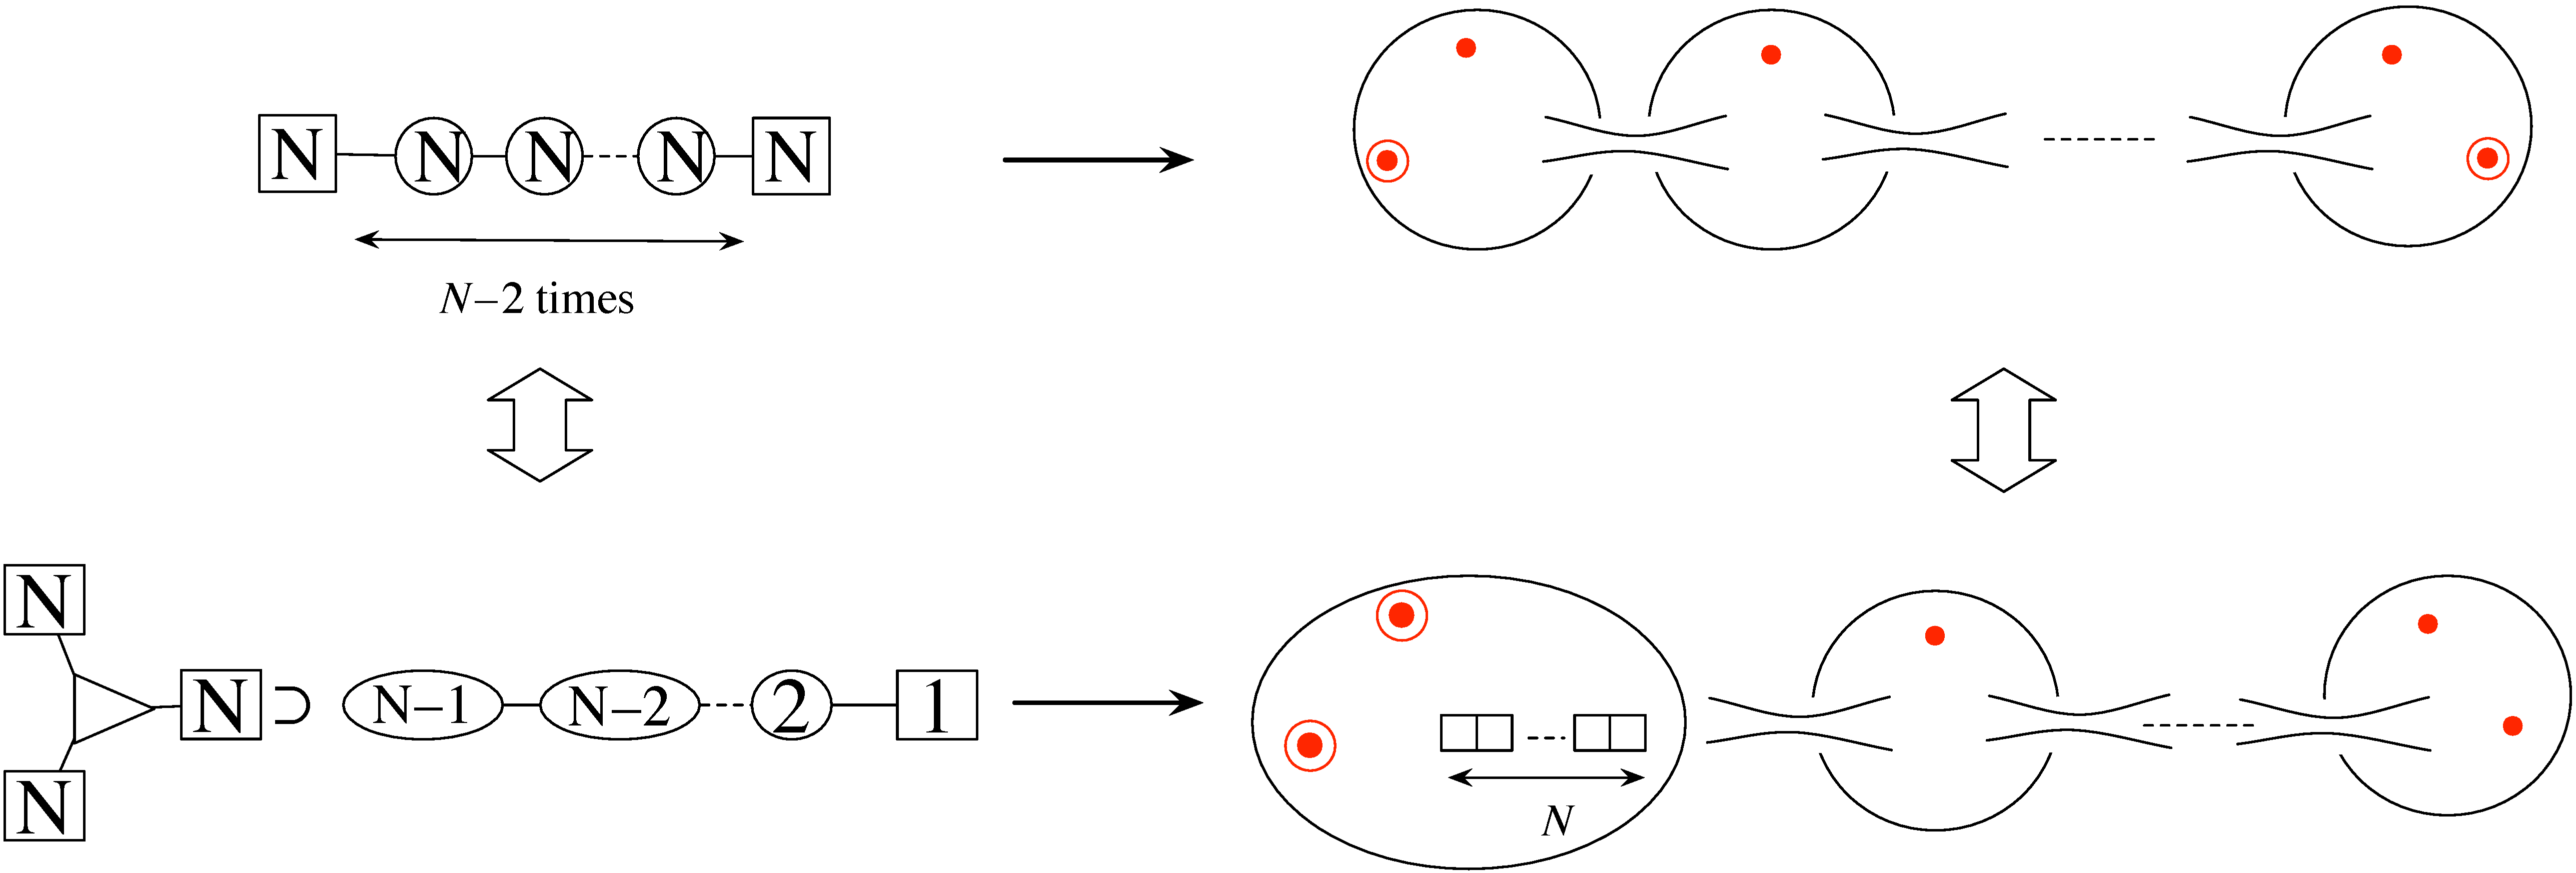
\includegraphics[width=\linewidth]{Tndual}}}
\]
\caption{产生 $T_N$ 理论的对偶。\label{fig:constructingTN}}
\end{figure}
现在可以愉快地摆弄一下穿孔了。例如，考虑规范群为 $\SU(N)^{N-2}$ 的规范理论，相邻群之间有双基本表示超多重态，首尾两个群还各有 $N$ 个额外的基本表示超多重态，见图 \ref{fig:constructingTN} 第一排。Seiberg-Witten 解很容易给出：它由 $\SU(N)$ 型理论的一个球面给出，带有两个完全穿孔和 $N-1$ 个简单穿孔。转到一个使这 $N-1$ 个简单穿孔全部退耦的对偶描述。应用第 \ref{sec:tame} 小节所学的退耦过程，得到规范群为
\begin{equation}
\SU(N-1)\times\SU(N-2)\times\cdots\SU(2),
\end{equation}
的箭图尾部，相邻两个群之间有双基本表示超多重态，最后的 $\SU(2)$ 还有一个二重态。第一个 $\SU(N-1)$ 规范化了类型为 $(1,1,\ldots,1)$ 的穿孔、即完全穿孔的味对称性 $\SU(N)$ 中的一个 $\SU(N-1)$ 子群。

\begin{figure}[h]
\[
\inc{Tn}
\]
\caption{$T_N$ 理论。\label{fig:TN}}
\end{figure}
通过这种方式，可以构造由带有三个完全穿孔的球面描述的理论。它称为 $T_N$ 理论，见图 \ref{fig:TN}。注意，$R_3=T_3$。由于有三个完全穿孔，味对称性至少为 $\SU(N)^3$。当 $N=3$ 时，前面已经看到，这一味对称性增强为 $E_6$。当 $N\ge4$ 时，原规范理论中不止有一个规范群。因此，不存在从 $\SU(N)\times\SU(N)$ 到其他群的增强。这与如下事实相符：当 $N\ge4$ 时，不存在一个包含 $\SU(N)^3$ 的群，使 $\SU(N)^2$ 增强为 $\SU(2N)$。将穿孔放在 $z=0,1,\infty$，可知 $\phi_k$ 具有形式
\begin{equation}
\phi_k=\frac{u_k^{(1)}+\cdots+u_k^{(k-2)}z^{k-3}}{z^{k-1}(z-1)^{k-1}}dz^k.
\end{equation}
因此，这一理论具有一个维数为 $3$ 的库仑支算符、两个维数为 $4$ 的库仑支算符，依此类推，直到 $N-2$ 个维数为 $N$ 的库仑支算符。

\begin{figure}[h]
\[
\begin{array}{c}
\inc{TnTn1}\\
\inc{TnTn2}
\end{array}
\]
\caption{相互耦合的 $T_N$ 理论副本的 S 对偶。\label{fig:TNTN}}
\end{figure}
现在，可以取两个 $T_N$ 理论的副本，并通过一个 $\SU(N)$ 规范多重态将它们耦合起来。在六维构造中，只是球面上有四个完全穿孔。因此，S 对偶结构与含有四个味的 $\SU(2)$ 理论完全相同，可以交换全部四个穿孔。事实上，$T_2$ 理论就是三基本表示超多重态 $Q_{ijk}$。

\subsubsection{$MN(E_7)$}\index{E7Theory@$E_7$ 理论|hyperpage}
\begin{figure}[h]
\[
\inc{E7dual}
\]
\caption{产生 $MN(E_7)$ 的对偶。\label{fig:constructingE7}}
\end{figure}
接下来，考虑图 \ref{fig:constructingE7} 中的对偶。最终得到一个三穿孔球面，带有两个完全穿孔和一个类型为 $(2,2)$ 的穿孔。在原规范理论中，有六个基本表示味耦合到 $\SU(4)$ 规范多重态，具有 $\SU(6)$ 味对称性。为了构造紫外曲线，将这六个味分为四个味和两个味，并应用图 \ref{fig:SUNtame} 第三排所示的规则。因此，三穿孔球面所代表的理论具有如下形式的味对称性 $F$：
\begin{equation}
\begin{array}{cccc}
F&\supset&\SU(6)&\times\SU(3)\\
\cup&&\cup\\
\SU(4)\times\SU(2)\times\SU(4)&\supset&\SU(4)\times\SU(2)\times\U(1)&\times\SU(3)
\end{array}.
\end{equation}

\begin{figure}[h]
\[
\inc{E7X}
\]
\caption{理论 $MN(E_7)$。\label{fig:E7}}
\end{figure}
幸而，这样的群 $F$ 唯一存在，即 $E_7$，见图 \ref{fig:E7}。当然，可以通过研究 $\phi_k(z)$ 来计算这一理论的库仑支算符数目。这里尝试另一种方法。原来的规范群是 $\SU(4)\times\SU(2)$，因此维数为 $2,3,4$ 的库仑支算符数目分别为 $2,1,1$。在对偶一侧，箭图尾部包含 $\SU(3)\times\SU(2)$，具有两个维数为 $2$ 的算符和一个维数为 $1$ 的算符。三穿孔球面所代表的理论应当补足差额。因此，它只有一个库仑支算符，维数为 $4$。这再次符合第 \ref{sec:rank-1SCFT} 小节宣称存在的一个秩为一的超共形理论的特征。它等价于 Minahan-Nemeschansky 理论 $MN(E_7)$。还可以像第 \ref{sec:AS} 小节末尾那样，检验流两点函数和希格斯支维数的一致性。
% [Tutor Note: p.159 原文 "two operators of dimension 2 and one operator of dimension 1" 中的 "dimension 1" 应为 "dimension 3"。判据：对偶一侧的箭图尾部为 $\SU(3)\times\SU(2)$，其库仑支算符的标度维数为 $\SU(3)$ 的 $2,3$ 与 $\SU(2)$ 的 $2$，即两个维数 $2$、一个维数 $3$；四维 $\cN{=}2$ 理论也不存在维数 $1$ 的库仑支算符。按此，三穿孔球面只需补足维数 $4$ 的那一个算符，与上下文的两组数目 $2,1,1$ 相符。正文照原文排版。]

\subsubsection{$MN(E_8)$}\index{E8Theory@$E_8$ 理论|hyperpage}
\begin{figure}[h]
\[
\inc{E8dual}
\]
\caption{产生 $MN(E_8)$ 理论的对偶。\label{fig:constructingE8}}
\end{figure}
现在，将它推广到 $E_8$ 对称性已经相当直接。进行图 \ref{fig:constructingE8} 所示的对偶变换。在对偶一侧，有一个三穿孔球面，带有一个完全穿孔、一个类型为 $(2,2,2)$ 的穿孔和一个类型为 $(3,3)$ 的穿孔。可知理论的味对称性 $F$ 应满足
\begin{equation}
\begin{array}{cccc}
F&\supset&\SU(5)&\times\SU(5)\\
\cup&&\cup\\
\SU(2)\times\SU(3)\times\SU(6)&\supset&\SU(2)\times\SU(3)\times\U(1)&\times\SU(5)
\end{array}.
\end{equation}
这与 Minahan-Nemeschansky 理论 $MN(E_8)$ 的结构吻合得很好，见图 \ref{fig:E8}。各种性质的检验留作读者练习。
\begin{figure}[h]
\[
\inc{E8X}
\]
\caption{$E_8$ 理论。\label{fig:E8}}
\end{figure}

\subsubsection{含有偶数个味的 $\SU(N)$ 理论的奇异极限}\label{sec:applicationL}\index{InfraredFreeTheory@红外自由理论|hyperpage}
最后，研究一个非共形的例子。考虑含有 $N_f=2n$ 个味的 $\SU(N)$ 理论，其中 $N>n$。曲线为
\begin{equation}
\frac{\Lambda^{N-n}\prod_{i=1}^n(x+\mu+\mu_i)}z
+\Lambda^{N-n}\prod_{i=1}^n(x+\mu+\tilde\mu_i)^nz
=x^N+u_2x^{N-2}+\cdots+u_N\label{Nn}
\end{equation}
微分为 $\lambda=xdz/z$。这里要求 $\sum_i\mu_i+\tilde\mu_i=0$，并将 $\U(1)$ 质量项单独记为 $\mu$。显然，当 $u_{N-n}=2\Lambda^{N-n}$ 时，$z\sim1$ 附近会发生一些事情。文献 \cite{Eguchi:1996vu} 最先考虑了这一点。正确的物理最初在文献 \cite{Gaiotto:2010jf} 中讨论。下面将看到，低能极限是一个与理论 $R_n$ 和 $X_{N-n+4}$ 耦合的红外自由 $\SU(2)$ 规范理论。

为了研究红外行为，令
\begin{equation}
u_{N-n,\text{old}}=2\Lambda^{N-n}+u_{N-n,\text{new}},\qquad z=1+\delta z
\end{equation}
并假定标度关系
\begin{equation}
\mu_i\sim\epsilon,\qquad
u_N\sim\epsilon^n,\quad u_{N-1}\sim\epsilon^{n-1},\quad\ldots,\quad u_{N-n+2}\sim\epsilon^2,\label{JJJ}
\end{equation}
以及
\begin{equation}
u_2\sim\epsilon'{}^2,\quad u_3\sim\epsilon'{}^3,\quad\ldots,\quad u_{N-n+2}\sim\epsilon'{}^{N-n+2}.
\end{equation}
于是，需要假定
\begin{equation}
\epsilon'{}^{N-n+2}\sim\epsilon^2.\label{ee}
\end{equation}
特别地，有
\begin{equation}
\epsilon\ll\epsilon'\ll1.
\end{equation}

在 $x\sim\epsilon$ 的区域中，可以将曲线 \eqref{Nn} 近似为
\begin{multline}
\frac{\Lambda^{N-n}\prod_{i=1}^n(x+\mu+\mu_i)}z
+\Lambda^{N-n}\prod_{i=1}^n(x+\mu+\tilde\mu_i)z\\
=(2\Lambda^{N-n}+u_{N-n})x^n+u_{N-n+2}x^{n-2}+\cdots+u_N
\end{multline}
并采用标度关系 \eqref{JJJ}。将它写成关于 $x$ 的 $n$ 次方程时，$x^n$ 项的系数为
\begin{equation}
\frac{\Lambda^{N-n}}z+\Lambda^{N-n}z-2\Lambda^{N-n}-u_{N-n}.\label{***}
\end{equation}
在极限 $\epsilon\to0$ 中，式 \eqref{***} 的两个零点在 $z=1$ 处碰撞。这正是第 \ref{sec:partII} 小节中，含有 $2n$ 个味的 $\SU(n)$ 理论在 $q\to1$ 极限下的情形。可以看到，得到的是与 $\SU(2)$ 规范群耦合的 $R_n$ 理论；算符 $u_{N-n+2}$ 现在被视为这一 $\SU(2)$ 的库仑支真空期望值。参数 $\mu_i$ 和 $\tilde\mu_i$ 现在是 $R_n$ 理论的 $\SU(2n)$ 对称性的质量参数。

在 $x\sim\epsilon'$ 的区域中，曲线 \eqref{Nn} 可以近似为
\begin{equation}
c\,\delta z^2=(x^{N-n}+u_2x^{N-n-2}+\cdots+\frac{u_{N-n+1}}x+\frac{u_{N-n+2}}{x^2}),
\end{equation}
其中微分 $\lambda=xd\delta z$，$c$ 是一个不重要的常数。在第 \ref{sec:ADAD} 小节已经遇到过它；它是描述含有两个味的 $\SU(N-n+1)$ 理论的 Argyres-Douglas 点的曲线。等价地，在第 \ref{sec:generalAD} 小节中将这一理论称为 $X_{N-n+4}$。

\begin{figure}[h]
\[
\inc{GSTX}
\]
\caption{含有 $N_f=2n$ 个味的 $\SU(N)$ 理论最奇异的点。\label{fig:EHIY}}
\end{figure}
总之，极限理论具有图 \ref{fig:EHIY} 所示的结构。具体而言，有一个弱耦合的 $\SU(2)$ 规范群，将 $x\sim\epsilon$ 的区域与 $x\sim\epsilon'$ 的区域连接起来：前者由 $\SU(n)$ 型六维理论的一个球面给出，代表 $R_n$ 理论；后者由 $\SU(2)$ 型六维理论的一个球面给出，代表理论 $X_{N-n+4}$。

在中间区域 $\epsilon'\gg x\gg\epsilon$ 中，曲线只是
\begin{equation}
\delta z^2\sim\frac{u_{N-n+2}}{x^2}
\end{equation}
微分为 $\lambda=\delta zdx\sim\sqrt{u_{N-n+2}}dx/x$。可见存在一个 $\SU(2)$ 规范群，且
\begin{equation}
a\sim\frac1{2\pi i}\oint\delta z\frac{dx}x\sim\sqrt{u_{N-n+2}}.
\end{equation}
于是，对偶坐标 $a_D$ 粗略地由下式给出：
\begin{equation}
a_D\sim\frac2{2\pi i}\int_{x\sim\epsilon'}^{x\sim\epsilon}\sqrt{u_{N-n+2}}\frac{dx}x
\sim\frac2{2\pi i}a\log\frac\epsilon{\epsilon'}.
\end{equation}
利用 $a\sim\epsilon$ 以及关系 \eqref{ee}，得到
\begin{equation}
a_D=\frac2{2\pi i}\frac{N-n}{N-n+2}a\log a+\cdots.
\end{equation}
回顾含有 $N_f$ 个味的 $\SU(2)$ 理论，其跑动由
\begin{equation}
a_D\sim\frac2{2\pi i}(4-N_f)a\log a+\cdots
\end{equation}
给出。因此，这一系统的有效味数为
\begin{equation}
N_f=\frac{5N-5n+8}{N-n+2}>4.
\end{equation}
现在 $\SU(2)$ 是红外自由的。注意，这正确地等于已经计算过的 $R_N$ 理论与 $X_{N-n+4}$ 理论的有效味数之和。确实，$R_N$ 理论的有效味数为 $3$，$X_{N-n+4}$ 理论的有效味数为 $2(N-n+1)/(N-n+2)$，分别见式 \eqref{k-of-su2} 和式 \eqref{GOO}。
\subsection{驯服穿孔与希格斯化}\label{sec:higgsing}\index{Higgsing@希格斯化|hyperpage}\index{NilpotentVev@幂零真空期望值|hyperpage}
\begin{figure}[h]
\[
\inc{partial-closing}
\]
\caption{穿孔类型的改变。\label{fig:partial-closing}}
\end{figure}

第 \ref{sec:tame} 小节以一种颇为临时性的方式，引入了紫外曲线上由杨图标记的穿孔。$\SU(4)$ 情形的例子展示在图 \ref{fig:SUNtame} 中。在本讲义最后一个小节里，我们希望稍微深入地研究杨图的意义。例如，应当如何理解图 \ref{fig:partial-closing} 中将完全穿孔变为简单穿孔、即类型为 $(3,1)$ 的穿孔的过程？本小节将始终以完全穿孔 $(1,1,1,1)$ 变为简单穿孔 $(3,1)$ 作为具体例子。推广到一般穿孔留作读者练习。本小节的内容基于作者与 Francesco Benini 在 2009 年至 2010 年间某时完成的一项未发表工作。

两者的 Seiberg-Witten 曲线都为
\begin{equation}
\lambda^4+\phi_2(z)\lambda^2+\phi_3(z)\lambda+\phi_4(z)=0.
\end{equation}
在两种情形中，$\phi_k(z)$ 都在 $z=0$ 处具有一个完全穿孔，在 $z=z_i$ 处具有五个简单穿孔。对于前者，$z=\infty$ 处原本是完全穿孔；对于后者，它是类型为 $(3,1,1)$ 的简单穿孔。

对于前者，场 $\phi_k(z)$ 为
\begin{equation}
\phi_k(z)=\frac{u_k^{(1)}+u_k^{(2)}z+u_k^{(3)}z^2+u_k^{(4)}z^3}{\prod_i^5(z-z_i)}\frac{dz^k}{z^{k-1}}.\label{former}
\end{equation}
对于后者，它们为
\begin{equation}
\begin{aligned}
\phi_2(z)&=\frac{u_2^{(1)}+u_2^{(2)}z+u_2^{(3)}z^2+u_2^{(4)}z^3}{\prod_i^5(z-z_i)}\frac{dz^2}z,\\
\phi_3(z)&=\frac{u_3^{(1)}+u_3^{(2)}z+u_3^{(3)}z^2}{\prod_i^5(z-z_i)}\frac{dz^3}{z^2},\\
\phi_4(z)&=\frac{u_4^{(1)}+u_4^{(2)}z}{\prod_i^5(z-z_i)}\frac{dz^4}{z^3}.
\end{aligned}\label{latter}
\end{equation}
这里，$u_k^{(i)}$ 是第 $i$ 个规范群的维数为 $k$ 的库仑支算符，根据极点结构确定它们的方法，已在式 \eqref{phifull} 附近说明。

显然，在式 \eqref{former} 中令 $u_4^{(3,4)}=u_3^{(4)}=0$，就得到式 \eqref{latter} 中的 $\phi_k(z)$。下面将解释，可以从第一个理论出发，将库仑支参数取在这一子空间上，然后移到希格斯支，从而实现第二个理论。

\begin{figure}[h]
\[
\inc{renaming-fields}
\]
\caption{为各场赋予新名称。\label{fig:renaming-fields}}
\end{figure}
为了便于分析希格斯支，为双基本表示引入新名称，见图 \ref{fig:renaming-fields}。将最右边的 $\SU(N)$ 味对称性命名为 $\SU(N)_0$，并从右向左将规范群命名为 $\SU(N)_{i=1,2,3,\ldots}$。为每个群引入一个辅助的 $N$ 维复空间 $V_i$。对于每一对相邻的 $\SU(N)_{i+1}\times\SU(N)_i$，有一个双基本表示超多重态 $(Q_b^a,\tilde Q_a^b)$，其中 $a=1,\ldots,N$ 和 $b=1,\ldots,N$ 分别是 $\SU(N)_{i+1}$ 与 $\SU(N)_i$ 的指标。将 $Q_b^a$ 视为线性映射 $A_i:V_i\to V_{i+1}$，将 $\tilde Q_a^b$ 视为反方向的映射 $B_i:V_{i+1}\to V_i$。注意，每一对 $(A_i,B_i)$ 都来自组成紫外曲线的若干三穿孔球面中的一个，如图所示。设总共有 $k$ 个三穿孔球面。

引入记号
\begin{equation}
M_i':=B_iA_i,\qquad\primeM_i:=A_iB_i.
\end{equation}
下面将反复使用显然的恒等式
\begin{equation}
\tr M_i'{}^n=\tr B_iA_i\cdots B_iA_i
=\tr A_iB_i\cdots A_iB_i=\tr{}\primeM_i{}^n.
\end{equation}

注意，$\tr M_i:=\tr M_i'=\tr\primeM_i$ 是第 $i$ 个 $\U(1)$ 味对称性的质量项，可以自然地与第 $i$ 个三穿孔球面的简单穿孔相联系。此外，还有另外两个规范不变组合，即
\begin{equation}
M_0'|_\text{traceless}:=M_0'-\frac1N\tr M_0,\qquad
\primeM_k|_\text{traceless}:=\primeM_k-\frac1N\tr M_k.
\end{equation}
$M_0'|_\text{traceless}$ 处于与最右侧球面在 $z=\infty$ 处的完全穿孔相联系的 $\SU(N)$ 味对称性的伴随表示中。类似地，$\primeM_k|_\text{traceless}$ 处于 $z=0$ 处穿孔的 $\SU(N)$ 味对称性的伴随表示中。

现在，我们希望通过给伴随表示场 $M_0'|_\text{traceless}$ 赋予非零真空期望值，对 $z=\infty$ 处的穿孔作局部修改。其他规范不变组合 $\tr M_i$（$i=1,\ldots,k$）和 $\primeM_k|_\text{traceless}$ “局域”在其他穿孔处。因此选择让它们保持为零。

来自 $\SU(N)_i$ 规范多重态中伴随表示标量的 F 项关系为
\begin{equation}
M_{i+1}'|_\text{traceless}={}\primeM_i|_\text{traceless}.
\end{equation}
由于施加了条件 $\tr M_i=0$，可以去掉取无迹部分的条件，直接写成
\begin{equation}
M_{i+1}'={}\primeM_i.
\end{equation}
于是，对任意 $n$，有如下关系：
\begin{equation}
\tr M_0'{}^n=\tr\primeM_0{}^n=\tr M_1'{}^n=\tr\primeM_1{}^n
=\cdots=\tr M_k'{}^n=\tr\primeM_k{}^n=0.
\end{equation}

这意味着，按 $\SU(N)$ 味对称性的伴随表示变换的规范不变组合 $M_0'$ 是一个幂零矩阵。可以通过复化的 $\SU(N)$ 旋转，将它化为 Jordan 标准形：
\begin{equation}
M_0'=J_{t_1}\oplus J_{t_2}\oplus\cdots,\qquad\sum_it_i=N\label{nilpotent-vev}
\end{equation}
其中 $J_t$ 是大小为 $t$ 的 Jordan 块，
\begin{equation}
J_t=\underbrace{\begin{pmatrix}
0&1\\
&0&1\\
&&0&1\\
&&&\ddots&\ddots\\
&&&&0
\end{pmatrix}}_t.
\end{equation}

再次得到了 $N$ 的一个分拆 $(t_i)$。下面将论证，这一分拆 $(t_i)$ 恰好就是第 \ref{sec:tame} 小节中用来标记穿孔的杨图。为了研究真空期望值 \eqref{nilpotent-vev} 的影响，需要找到一组满足 F 项和 D 项关系的超多重态场 $(A_i,B_i)$ 的取值。

\begin{figure}[h]
\[
\inc{more-notation}
\]
\caption{矩阵的图示记号。\label{fig:more-notation}}
\end{figure}
为了写出这样一组取值，再引入一种图示记号很有用，见图 \ref{fig:more-notation}。$N$ 维向量空间 $V$ 具有 $N$ 个基向量，用一列 $N$ 个点来表示它们。从 $V$ 到 $V'$、矩阵元为 $0$ 或 $1$ 的矩阵，可以用一组箭头表示：当且仅当矩阵的第 $(a,b)$ 元为 $1$ 时，从 $V$ 的第 $a$ 个点向 $V'$ 的第 $b$ 个点画一条箭头。图 \ref{fig:more-notation} 中间表示了大小为 $4$ 的 Jordan 块 $J_4$。同一图最右侧的图示表示投影到最后两个基向量的投影算符。

\begin{figure}[h]
\[
\inc{Higgsing}
\]
\caption{希格斯支上的一个特定点。\label{fig:higgsing}}
\end{figure}
为明确起见，令 $N=4$，并给 $M_0'$ 赋予类型为 $(3,1)$ 的幂零真空期望值，即由 $J_3\oplus J_1$ 给出。图 \ref{fig:higgsing} 给出 F 项关系的一个解。从中可以看到，此时未破缺的规范群为 $\SU(4)\times\SU(4)\times\SU(3)\times\SU(2)$。

一般而言，可以如下构造 F 项关系的解。假设希望令 $M_0'=X$，其中 $X$ 处于 Jordan 标准形。将向量空间作等同 $V_0=V_1=V_2=\cdots$。引入记号 $W_i=\Im X^i$，并将到 $W_i$ 的投影算符记为 $P_{W_i}$。然后令
\begin{equation}
A_0=X,\quad A_1=XP_{W_1},\quad A_2=XP_{W_2},\ldots
\end{equation}
并取
\begin{equation}
B_0=P_{W_1},\quad B_1=P_{W_2},\quad B_2=P_{W_3},\ldots.
\end{equation}
显然，剩余规范群具有形式
\begin{equation}
\cdots\times\SU(N_3)\times\SU(N_2)\times\SU(N_1)
\end{equation}
其中
\begin{equation}
N_i=N-\dim W_i=N-\rank X^i.
\end{equation}
定义 $s_i=N_i-N_{i-1}$。简短的组合计算表明：当 $X$ 的类型由一个从左数第 $i$ 列高度为 $t_i$ 的杨图描述时，序列 $(s_1,s_2,\ldots)$ 中的 $s_i$ 就是从下往上数第 $i$ 行的宽度。这正是第 \ref{sec:tame} 小节已经引入的规范群规则。现在来确定所得理论的无质量物质内容。

一种间接但迅速的确定物质内容的方法如下。我们从一个不含任何参数的超共形理论出发。希格斯化之后，唯一具有质量量纲的参数是超多重态场的真空期望值。根据第 \ref{sec:hypergeneral} 小节讨论过的拉格朗日量中超多重态部分与矢量多重态部分的一般退耦性质，希格斯化之后的低能理论中不能出现任何质量项或动力学能标。因此，所得理论也是超共形的。已经确定了 $N_i$，而且只能存在双基本表示场或基本表示场。这表明，$\SU(N_i)$ 应当恰好具有
\begin{equation}
n_i=2N_i-N_{i+1}-N_{i-1}\label{additional-funds}
\end{equation}
个额外的基本表示超多重态。

\begin{figure}[h]
\[
\inc{mass-term}
\]
\caption{为标量场产生的质量项。\label{fig:mass-term}}
\end{figure}
当然，这一结果也可以通过直接计算系统中各个场的质量项得到。注意，原来存在 $\cN{=}1$ 超势 $\tr A_i\Phi_iB_i$ 和 $\tr B_i\Phi_{i+1}A_i$，其中 $\Phi_i$ 是 $\SU(N)_i$ 矢量多重态中的伴随表示标量。由于给 $A_i$ 与 $B_i$ 的某些分量赋予了真空期望值，三点耦合会使超多重态标量与矢量多重态标量的某些分量配对。图 \ref{fig:mass-term} 展示了一个例子。其中，用向左下方的箭头表示的 $A_1$ 的真空期望值，使对应于 $V_2$ 的规范群的矢量多重态标量的一个分量与 $B_1$ 的一个分量之间产生质量项。

\begin{figure}[h]
\[
\inc{remaining-fields}
\]
\caption{希格斯化后剩下的场。\label{fig:remaining-fields}}
\end{figure}
可以看到，始终有一个 $\SU(N_{i+1})\times\SU(N_i)$ 的双基本表示保持无质量。但是，仔细分析质量项后会发现，有时还有更多带荷超多重态保持无质量。例如，如图 \ref{fig:remaining-fields} 所示，$V_3$ 与 $V_2$ 之间的整个双基本表示都保持无质量。在 $V_2$ 处，$\SU(4)$ 破缺到 $\SU(3)$。因此，从 $V_3$ 处未破缺的 $\SU(4)$ 的观点看，存在一个 $\SU(4)\times\SU(3)$ 双基本表示，以及一个 $\SU(4)$ 基本表示。将这一分析推广，就可以看出 $\SU(N_i)$ 的额外基本表示超多重态数目由式 \eqref{additional-funds} 给出。

\begin{figure}[h]
\[
\inc{flavor-telekinesis}
\]
\caption{味对称性的分配。\label{fig:flavor-telekinesis}}
\end{figure}

第 \ref{sec:tame} 小节曾说，$z=\infty$ 处的穿孔承载了与连接到 $\SU(N_i)$ 的额外 $n_i$ 个基本表示超多重态相关的全部味对称性。这听起来多少有些违背直觉，因为味对称性 $\SU(n_i)$ 看上去更应与第 $i$ 个节点相联系。现在可以理解这里起作用的物理机制了。为明确起见，再取类型为 $(3,1)$ 的穿孔，见图 \ref{fig:flavor-telekinesis}。根据我们的规则，真空期望值 $X=M_0'$ 为 $X=J_3\oplus J_1$；它在作用于三个基向量的 $\U(1)$ 旋转下不变，这三个基向量用图中的黑点表示。如果不伴随规范旋转，这一对称性并不保持希格斯真空期望值 $\vev{A_i}$ 和 $\vev{B_i}$ 不变。为了使对称性与希格斯真空期望值相容，需要同时旋转其他所有基向量：它们通过代表 $A_i$ 和 $B_i$ 的箭头，与原来的黑点相连接。

可以看到，希格斯真空期望值将旋转 $V_0$ 的三个基向量的 $\U(1)$ 味对称性，与旋转 $V_3$ 最后一个基向量的 $\U(1)$ 味对称性对应起来。希格斯化之后，后一个 $\U(1)$ 对称性恰好就是 $V_3$ 处 $\SU(4)$ 的额外一个基本表示超多重态所承载的味对称性，图中用实心三角形表示。这一分析可以推广到任意类型的穿孔。

总之，我们找到了对第 \ref{sec:tame} 小节引入的穿孔的一种新解释。这样的穿孔始终可以从完全穿孔得到：先将库仑支真空期望值选在适当的子空间上，再给超多重态组合 $M_0'$ 赋予幂零真空期望值；$M_0'$ 按与完全穿孔相联系的味 $\SU(N)$ 的伴随表示变换。赋予 $M_0'$ 的真空期望值，使某些 $i>0$ 的其他超多重态场 $A_i$、$B_i$ 获得非零真空期望值，从而将原规范群 $\cdots\times\SU(N)\times\SU(N)\times\SU(N)$ 破缺为 $\cdots\times\SU(N_3)\times\SU(N_2)\times\SU(N_1)$。
